\section{Обеспечение безопасных условий труда инженера-программиста при проведении исследования многослойных перцептронов для сжатия изображений}

При проведении исследований в области сжатия данных и изучении свойств нейронных сетей используется электронно-вычислительная техника.
Исследование включает в себя поиск и анализ материалов по использованию нейронных сетей в качестве способа сжатия графической информации.
Процесс исследования тесно связан с необходимостью восприятия изображений на экране, наблюдением за изменениями в системе, ведением записей, подготовкой чтением рукописных и печатных материалов.

Зрительное восприятие человека является одним из основных в системе анализаторных систем.
В процессе работы с персональной электронной вычислительной машиной(ПЭВМ) можно столкнуться с такими вредными факторами: несоответствие визуальных эргономических параметров дисплея (по яркости, контрасту, цветовой гамме и т. д.); неправильное расположение рабочих мест; неправильно спроектированное освещение в помещении.

Рабочее место необходимо располагать таким образом, чтобы в поле зрения не попадали оконные проемы или осветительные приборы. Следует добиваться уменьшения отражений на экране от различных источников света.

При низком уровне освещенности ухудшается видимость, при слишком высоком - уменьшается контраст изображения на экране.
Освещенность на поверхности стола в зоне размещения рабочего документа должна быть 300-500 лк.
Возможна установка светильников местного освещения для подсветки документов.
При этом не следует допускать появления бликов на экране и увеличения его освещенности - более 300 лк~\cite{ot_electric_lighting}.

В зависимости от источников света производственное освещение может быть естественным, искусственным и совмещенным.
Естественное освещение создается источниками света природного характера.
Освещение обеспечивается через оконные проемы с коэффициентом естественного освещения КЕО не ниже 1,2\% в зонах с устойчивым снежным покровом и не ниже 1,5\% на остальной территории~\cite{ot_electric_lighting}.

Искусственное освещение создается лампами накаливания, люминесцентными лампами или источниками, использующие светодиоды.
Искусственное освещение в помещениях эксплуатации компьютеров должно осуществляться системой общего равномерного освещения.
Совмещенное освещение представляет собой дополнение естественного освещения искусственным в темное и светлое время суток при недостаточном естественном освещении.
Искусственное освещение делится на несколько разновидностей: общее; местное; комбинированное.
При общем освещении происходит равномерное распределение света по все площади.
Это достигается соблюдением одинакового расстояния между светильниками, которые равномерно рассеянны.

При источнике света, локализованном в одной точке, будет наблюдаться разница в яркости света, но резкие перепады будут отсутствовать.
Примером может послужить расположенная посередине потолка люстра.

Чтобы выделить необходимые объекты или зоны используют местное освещение.
Источник света при этом располагают на определенном участке: рабочем столе или части стены.
В нашем случае это настольные лампы, расположенные на каждом рабочем столе.

Естественное освещение желательно осуществлять через светопроемы, ориентированные преимущественно через север и северо-восток.

\begin{figure}[ht]
\centering
  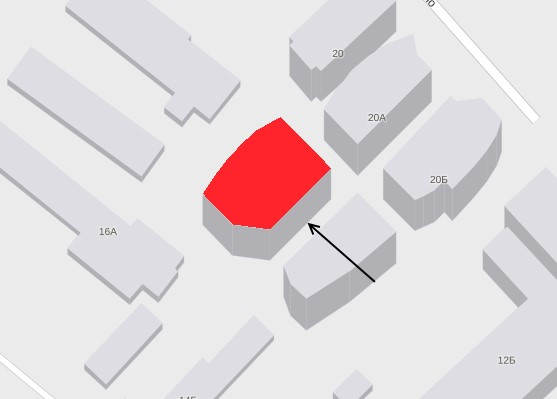
\includegraphics[scale=0.85]{ot_office_position.jpg}
  \caption{ Расположение окон офиса относительно сторон света }
  \label{fig:office_position}
\end{figure}

На (рисунок~\ref{fig:office_position}) видно, что светопроемы направлены на юго-восток, поэтому могут возникать проблемы, когда в дневное время суток, прямые солнечные лучи будут попадать на рабочее место, и вызывать блики на поверхности дисплея.
Рекомендуется установить жалюзи, чтобы контролировать поток солнечного света.

\begin{figure}[ht]
\centering
  
\includegraphics[scale=0.85]{ot_office_lamp.jpg}
  \caption{ Офисный светодиодный светильник }
  \label{fig:office_lamp}
\end{figure}

В качестве источников света при искусственном освещении должны применяться преимущественно люминесцентные лампы.
В данном случае используется освещение общее освещение, создаваемое светодиодными лампами (рисунок~\ref{fig:office_lamp}).
В сравнение с обычными лампами накаливания, а также люминесцентными лампами светодиодные источники света обладают многими преимуществами~\cite{ot_diod_lamp}.

Экономично используют энергию по сравнению с предшествующими поколениями электрических источников света --- дуговыми, накальными и газоразрядными лампами.
Так, световая отдача светодиодных систем уличного освещения с резонансным источником питания достигает 120 люмен на ватт, что сравнимо с отдачей люминесцентных ламп --- 60-100 люмен на ватт.
Для сравнения, световая отдача ламп накаливания, включая галогенные, составляет 10—24 люмен на ватт~\cite{ot_diod_lamp}.

При оптимальном подключении источников питания, применении качественных компонентов и обеспечении надлежащего теплового режима срок службы светодиодных систем освещения при сохранении приемлемых для общего освещения показателей может достигнуть 36—72 тысяч часов, что в среднем в 50 раз больше по сравнению с номинальным сроком службы ламп накаливания общего назначения и в 4—16 раз больше, чем у большинства люминесцентных ламп.

Отсутствие инерционности при включении и выключении, что важно для светодинамических установок.
Возможность диммирования по сравнению с большинством типов люминесцентных ламп.
Отсутствие в составе соединений ртути (в отличие от газоразрядных люминесцентных ламп и других приборов), что исключает отравление ртутью при переработке и при эксплуатации.
Практически полное отсутствие ультрафиолетового и инфракрасного излучения~\cite{ot_russia_encyclopedia}.

К недостаткам светодиодного освещения можно отнести: Спектр светодиодной лампы отличается от солнечного, поэтому приходится идти на компромисс между световой мощностью и качеством. Вместе с тем, он зачастую, при правильно подобранных люминофорах лучше по сравнению с люминесцентными лампами.

\begin{figure}[ht]
\centering
  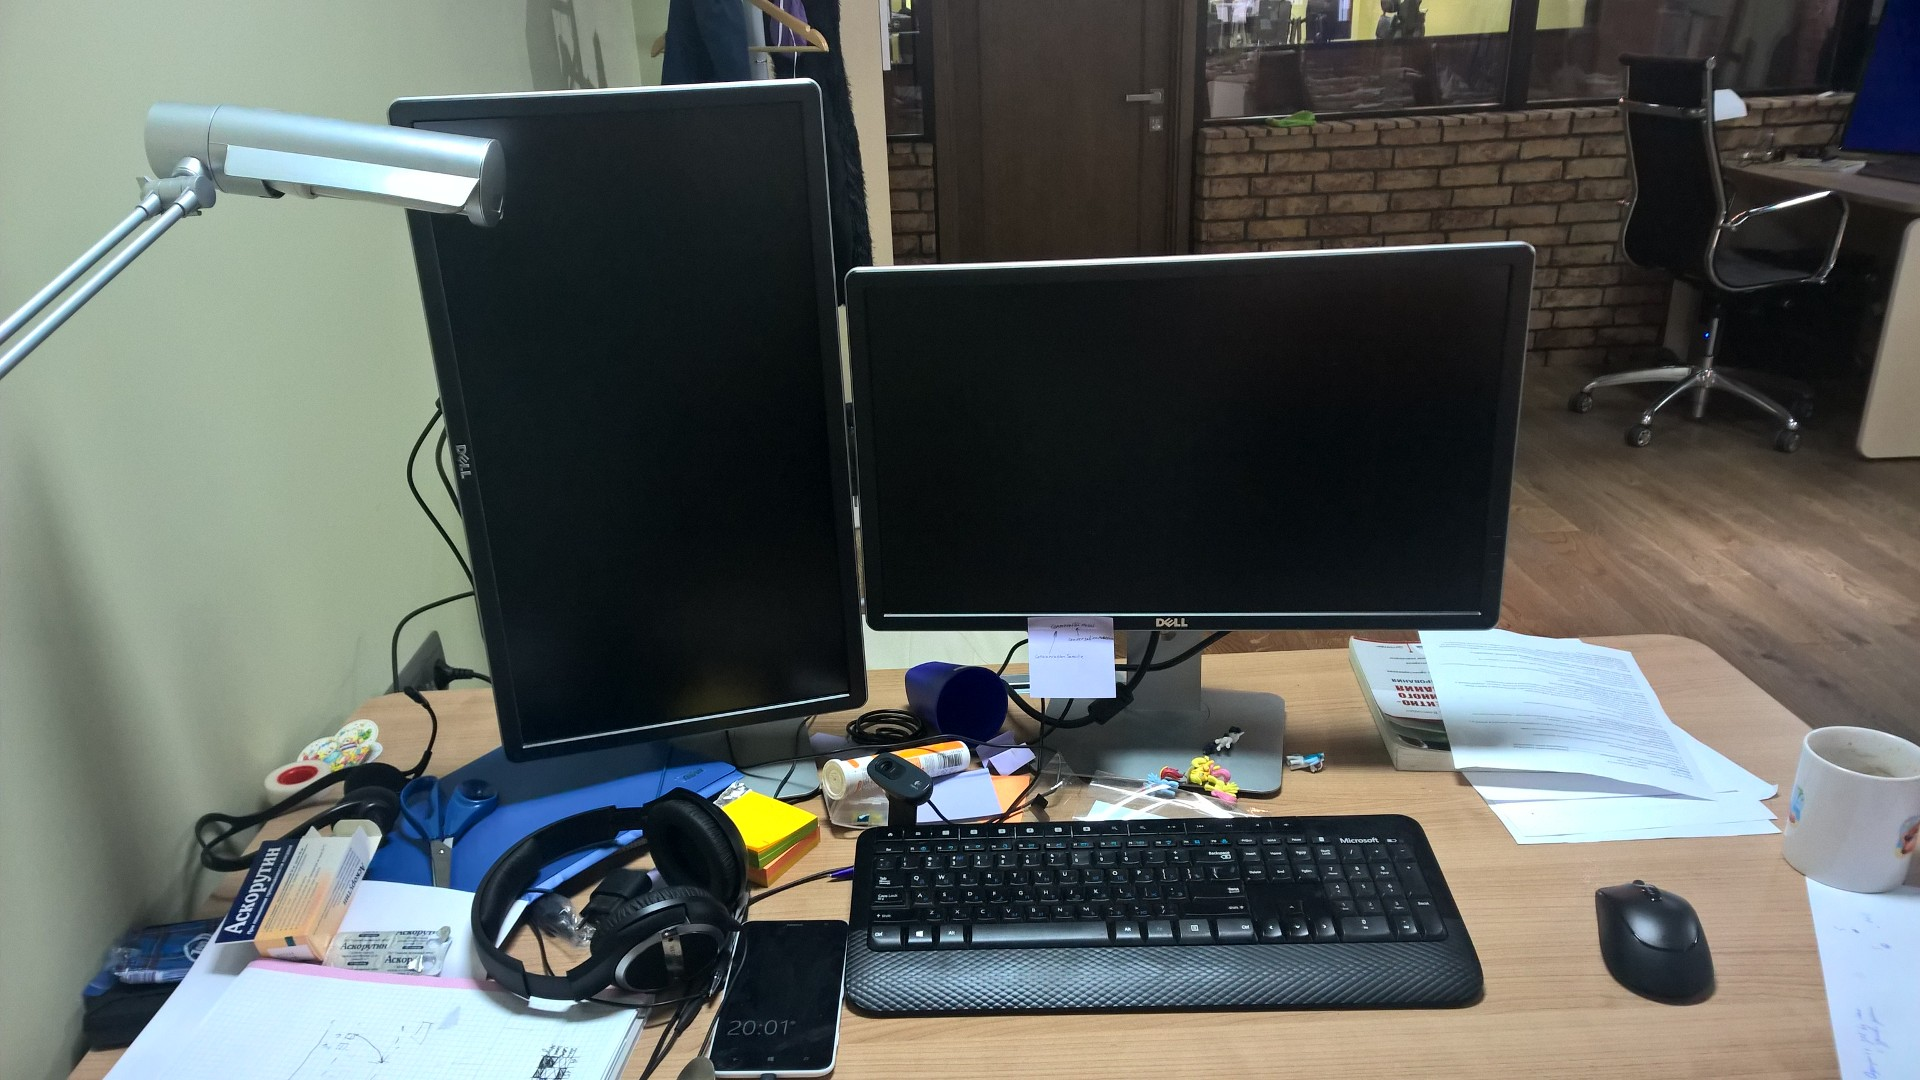
\includegraphics[scale=0.16]{ot_office_desktop.jpg}
  \caption{ Рабочее место }
  \label{fig:office_desktop}
\end{figure}

Рабочее место также оборудовано местным освещением в виде светильника с установленной компактной люминесцентной лампой мощность 20 ватт(рисунок~\ref{fig:office_desktop}).
Лампа имеет цветовую температуру дневного света 4200 К.
Местное освещении требуется при длительной работе с печатными источниками информации.
Рабочее место размещается таким образом, чтобы естественный свет падает сзади, что создает неудобства при работе ранним утром.
Светильники общего освещения создают нормальные условия освещенности и соответствующий контраст между экраном и окружающей обстановкой с учетом вида работы и требований видимости со стороны работника.
На рабочем месте используются мониторы с матовым покрытием, поэтому даже с ярким искусственным или естественным освещением работа с ним не доставляет дискомфорта.
Возможные мешающие отражения и отблески на экране монитора и другом оборудовании устраняются путем соответствующего размещения экрана, оборудования, расположения светильников местного освещения.

Проблемы связанные с бликами на экране ранним утром решаются закрытием жалюзей или поворотом рабочего места боком к световым проемам.
Таким образом, изложенные выше предложения обеспечивают безопасность условий труда инженера программиста при проведении исследования по теме «Многослойные перцептроны для сжатия изображений».
